\chapter{BACK END}
    \section{Cấu trúc hệ thống}
        \subsection{Mô hình Client - Server}
            \begin{figure}[H]
                \centering
                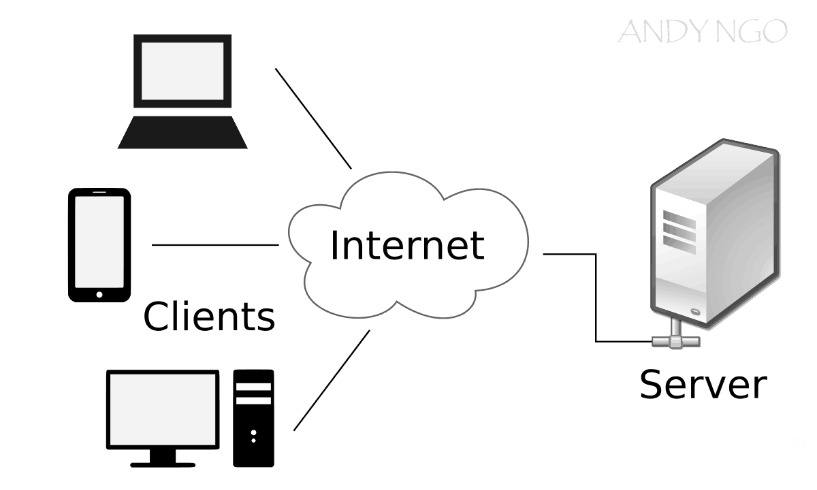
\includegraphics[width=0.8\textwidth]{pictures/ServerClient.png}
                \caption{Mô hình Client - Server}
                \label{fig:client-server}
            \end{figure}
            \hspace*{0.6cm}Mô hình Client - Server là một mô hình kiến trúc mạng trong đó các ứng dụng được chia thành hai phần: client và server. Client là phần mềm chạy trên máy tính của người dùng, trong khi server là phần mềm chạy trên máy chủ. Client gửi yêu cầu đến server và nhận phản hồi từ server.
        \subsection{Kiến trúc RESTful API}
            \hspace*{0.6cm}Kiến trúc RESTful API là một kiểu kiến trúc phần mềm cho phép các ứng dụng giao tiếp với nhau thông qua HTTP. RESTful API sử dụng các phương thức HTTP như GET, POST, PUT, DELETE để thực hiện các thao tác CRUD (Create, Read, Update, Delete) trên tài nguyên.
            \begin{figure}[H]
                \centering
                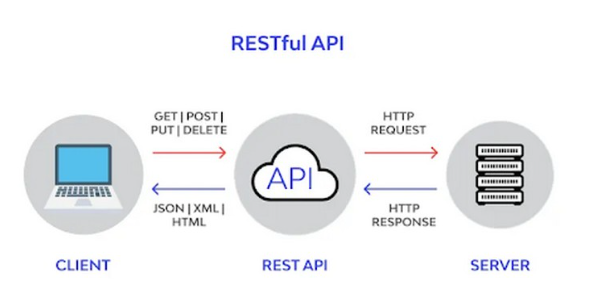
\includegraphics[width=0.8\textwidth]{pictures/RESTfulAPI.png}
                \caption{Kiến trúc RESTful API}
                \label{fig:restful-api}
            \end{figure}
        \subsection{Mô hình MVC}
            \hspace*{0.6cm}Mô hình MVC (Model-View-Controller) là một mô hình thiết kế phần mềm được sử dụng phổ biến trong phát triển ứng dụng web. Mô hình này chia ứng dụng thành ba phần: Model (mô hình), View (giao diện) và Controller (bộ điều khiển). Mỗi phần có nhiệm vụ riêng và tương tác với nhau để tạo ra ứng dụng hoàn chỉnh.
            \begin{figure}[H]
                \centering
                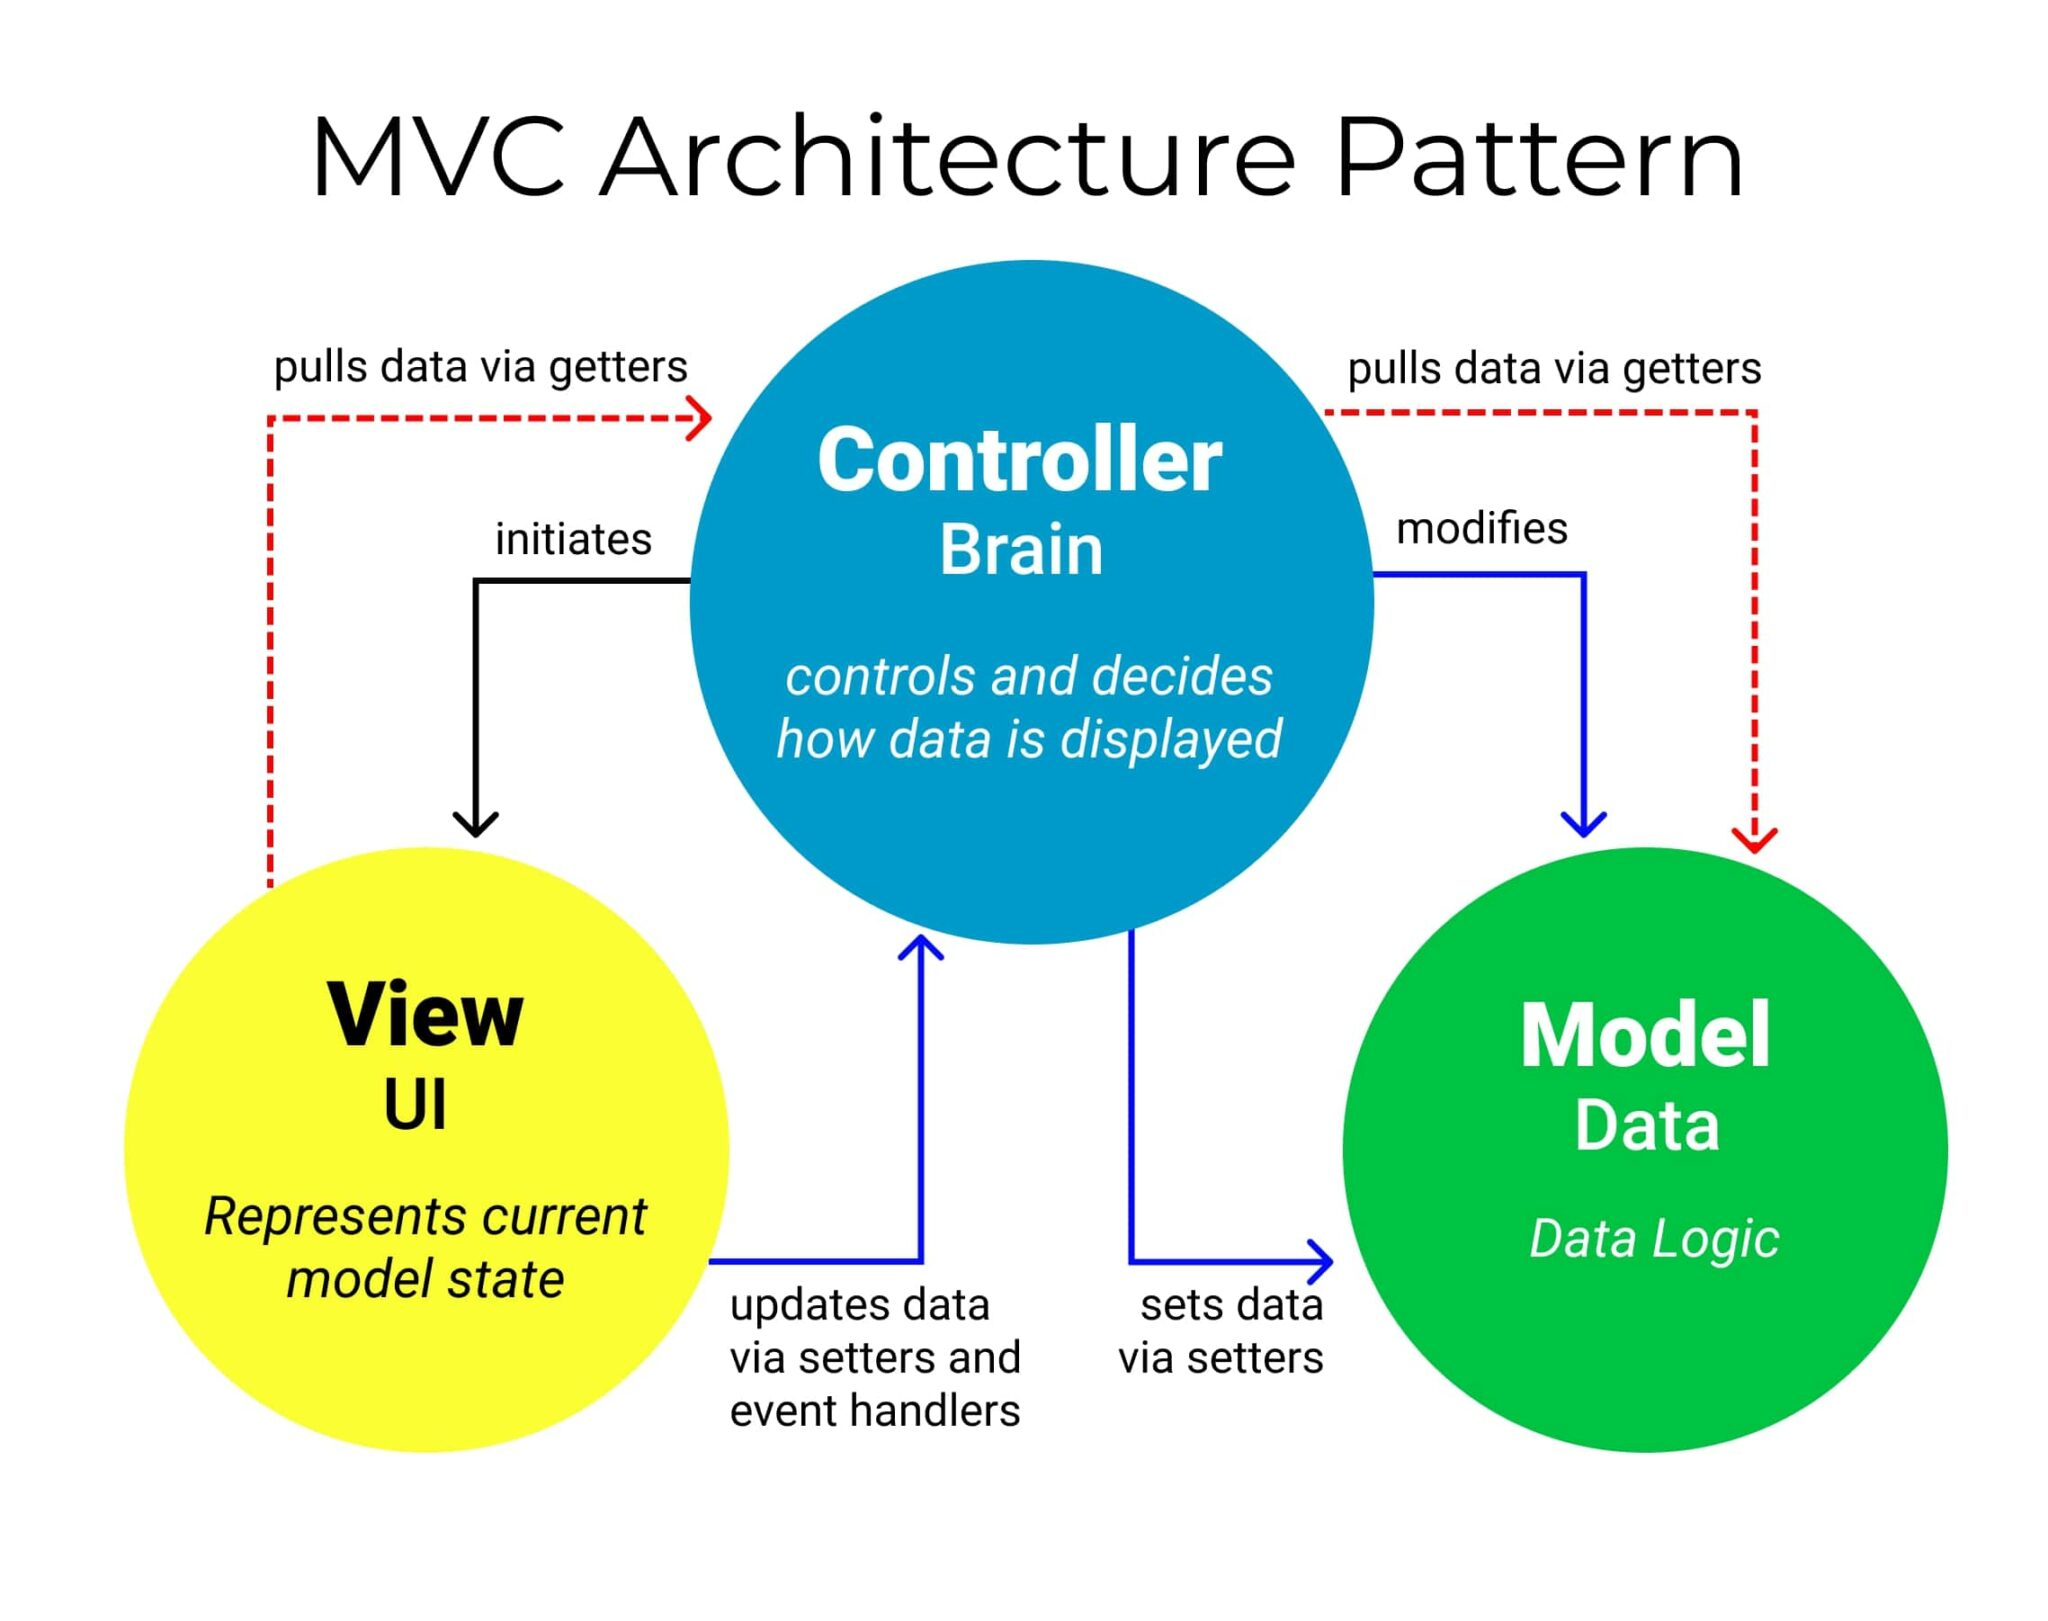
\includegraphics[width=0.8\textwidth]{pictures/MVC.png}
                \caption{Mô hình MVC}
                \label{fig:mvc}
            \end{figure}
        \subsection{Kiến trúc Layered}
            \hspace*{0.6cm}Kiến trúc Layered là một kiểu kiến trúc phần mềm trong đó ứng dụng được chia thành nhiều lớp. Mỗi lớp có nhiệm vụ riêng và tương tác với các lớp khác thông qua các giao diện. Kiến trúc Layered giúp tách biệt các phần của ứng dụng, dễ dàng bảo trì và mở rộng. Ở đây chúng ta có:
            \begin{itemize}
                \item Presentation Layer: Front-end.
                \item Application Layer: mainServer
                \item Data Layer: dbServer và MongoDB.
            \end{itemize}
            \begin{figure}[H]
                \centering
                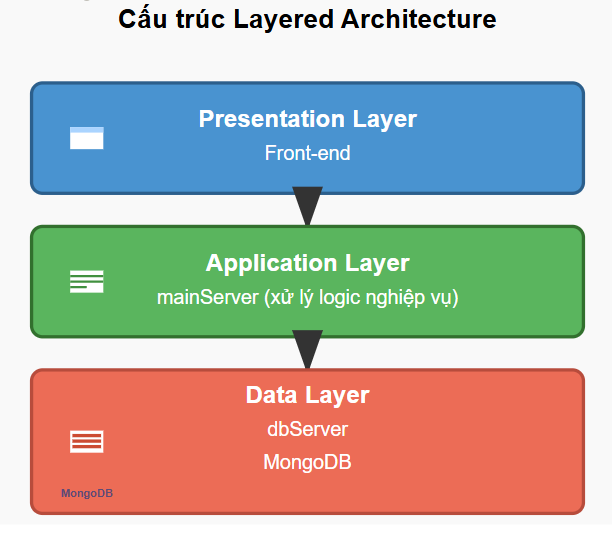
\includegraphics[width=0.8\textwidth]{pictures/Layered.png}
                \caption{Kiến trúc Layered}
                \label{fig:layered}
            \end{figure}
    \section{Cấu trúc thư mục}
        \hspace*{0.6cm}Cấu trúc thư mục của dự án được tổ chức như sau:
        \begin{itemize}
            \item mainServer: Thư mục chứa mã nguồn của Main Server.
            \begin{itemize} 
                \item controllers: Thư mục chứa các controller.
                \item middlewares: Thư mục chứa các middleware.
                \item routes: routes: Thư mục chứa các route.
                \item upload: Thư mục chứa các tệp tải lên.
                \item server.js: Tệp chính của Main Server.
            \end{itemize}
            \item dbServer: Thư mục chứa mã nguồn của Database Server.
            \begin{itemize}
                \item config: Thư mục chứa các tệp cấu hình.
                \item models: Thư mục chứa các mô hình dữ liệu.
                \item seeds: Thư mục chứa các tệp khởi tạo dữ liệu.
                \item dbserver.js: Tệp chính của Database Server.
            \end{itemize}
            \item .env: Tệp cấu hình môi trường.
        \end{itemize}
    \section{Cài đặt}
        \hspace*{0.6cm}Các bước khởi tạo server:
        \begin{itemize}
            \item Khởi tạo NodeJS: \texttt{npm init -y}
            \item Cài đặt dependencies:
            \begin{itemize}
                \item Express: \texttt{npm install express}
                \item Mongoose: \texttt{npm install mongoose}
                \item Multer: \texttt{npm install multer}
                \item Dotenv: \texttt{npm install dotenv}
                \item Cors: \texttt{npm install cors}
                \item Bcrypt: \texttt{npm install bcrypt}
                \item Jsonwebtoken: \texttt{npm install jsonwebtoken}
            \end{itemize}
            \item Tạo server chính: \texttt{touch server.js} và \texttt{touch dbserver.js}
            \item Chạy server bằng lệnh: \texttt{npm start} 
        \end{itemize}
        \hspace*{0.6cm}Các thư viện khác cài đặt trong quá trình phát triển.